% !TeX TXS-program:bibliography = txs:///biber

\documentclass[
    paper=a4,
    fontsize=10pt,
    DIV=13,
    % twocolumn,
    oneside,
]{scrartcl}

%-------------------------------------------------------------------------------------------------
%   Packages, Style Guide
%-------------------------------------------------------------------------------------------------

%-------------------------------------------------------------------------------------------------
%   Packages
%-------------------------------------------------------------------------------------------------

\usepackage[utf8]{inputenc}                         % utf8 as input encoding
\usepackage[T1]{fontenc}                            % 8bit font encdoing
\usepackage[ngerman]{babel}                         % word seperation
\usepackage{microtype}                              % font expansion
\usepackage{libertine}                              % select font
\usepackage[libertine]{newtxmath}                   % select font for mathmode
\usepackage{scrlayer-scrpage}                       % Bessere Kopfzeilen

\usepackage[
    locale=DE,
    detect-all,
    per-mode=fraction,
]{siunitx}                                          % express SI units
\usepackage{amsmath}
\usepackage{booktabs}                               % better tables
\usepackage{tabularx}                               % tables with pagewidth
\usepackage{graphicx}                               % input pictures
\usepackage{svg}
\usepackage{xcolor}
\usepackage{flushend}
\usepackage{listingsutf8}

\usepackage{csquotes}                               % quote environment
\usepackage[
    backend=biber,
    style=ieee,
]{biblatex}                                          % source control

\usepackage{hyperref}                               % add hyperlinks

%-------------------------------------------------------------------------------------------------
%   Colors
%-------------------------------------------------------------------------------------------------

% \definecolor{colorblue}{HTML}{0480CC}				% color for weblinks
% \definecolor{colordarkblue}{HTML}{4C1DCC}			% no use case at the moment
% \definecolor{colorgreen}{HTML}{26CC1B}				% color for citations
% \definecolor{colorred}{HTML}{CC1204}				% color for pdf links
\definecolor{coloryellow}{HTML}{F0B707}			    % color for warnings

%-------------------------------------------------------------------------------------------------
%   Lengths
%-------------------------------------------------------------------------------------------------

\newlength{\imagewidth}
\setlength{\imagewidth}{0.7\columnwidth}

%-------------------------------------------------------------------------------------------------
%   Style Options
%-------------------------------------------------------------------------------------------------

\KOMAoptions{
    toc     =   listof,                                     % add table of figures in 
    % headsepline=true,                               % switch header rule
    numbers =   noendperiod,
}

\hypersetup{
    colorlinks=true,
    bookmarksnumbered=true,
}

\chead{Laborbericht Regelungstechnik}
\ohead{Versuch Nr. \printlabor}
\ihead{Jan Hoegen}

\flushbottom                                        % fill pages to bottom

\addbibresource{quellen.bib}

%-------------------------------------------------------------------------------------------------
%   Macros
%-------------------------------------------------------------------------------------------------
        
\newcommand{\missing}{%
    \textcolor{coloryellow}{MISSING}%
    \PackageWarning{rtl_labor}{You used the 'missing' macro at this line. Remove it before finalising document}%
}
\newcommand{\improve}{%
    \textcolor{coloryellow}{IMPROVE}%
    \PackageWarning{rtl_labor}{You used the 'improve' macro at this line. Remove it before finalising document}%
}

\newcommand{\legend}[1]{\par\footnotesize\textbf{Legende}: #1\par}
\newcommand{\figsource}[1]{\par\footnotesize\textbf{Quelle:} #1\par}

%-------------------------------------------------------------------------------------------------
%   Title Page
%-------------------------------------------------------------------------------------------------

\titlehead{%
    Hochschule Karlsruhe\\
    University of Applied Sciences\\
    Fakultät für Elektro- und Informationstechnik
}
\title{Laborbericht Regelungstechnik}

\publishers{Betreuer: Prof. Dr. Keller}

\author{%
    Jan Hoegen\thanks{%
        Matrikel-Nr. 82358. E-Mail \href{jan.hoegen@web,de}{jan.hoegen@web,de}}%
    % \and%
    % Rithik Kurmar\thanks{%
    %     Matrikel-Nr. . E-mail \href{}{}}
}

\newcommand{\labor}[1]{\newcommand{\printlabor}{#1}}

\AtBeginDocument{
    \subtitle{Versuch Nr.~\printlabor}
    
    \hypersetup{
        pdftitle = {RT Labor \printlabor\ | Hoegen},
    }
}

%-------------------------------------------------------------------------------------------------
%   Listing Settings
%-------------------------------------------------------------------------------------------------

\lstset{%
	frame			=	tb ,							%	horizontale Linie oben&unten
	breaklines		=	true,							%	Zeilenumbruch
	rulecolor		=	\color{black} ,					%	Rahmenfarbe ist schwarz
	% keywordstyle	=	\keywordcolor ,
	% commentstyle	=	\commentcolor ,
	% stringstyle		=	\stringcolor ,
	title			=	\lstname ,						%	Titel ist gleich dem Dateinamen
	basicstyle		=	\footnotesize\ttfamily ,		%	Kleine Schrift und Monospace
	% numbers			=	right,							%	Zeilennumber rechts (da marginalie links)
	inputencoding	=	utf8,  							% Input encoding
    extendedchars	=	true,  							% Extended ASCII
}
% \lstdefinestyle{TeX}{language=TeX,						%	Mehr Keywörter für TeX
%     morekeywords={vspcae, hspace, rule, ifdefined, newcommand, setlength, newlentgh, RequirePackage, ProvidesPackage, NeedsTexFormat, DeclareOption, ProcessOption}, 
% }
\lstset{literate=							%	ermöglicht Unicode-Zeichen in Listing!
  {á}{{\'a}}1 {é}{{\'e}}1 {í}{{\'i}}1 {ó}{{\'o}}1 {ú}{{\'u}}1
  {Á}{{\'A}}1 {É}{{\'E}}1 {Í}{{\'I}}1 {Ó}{{\'O}}1 {Ú}{{\'U}}1
  {à}{{\`a}}1 {è}{{\`e}}1 {ì}{{\`i}}1 {ò}{{\`o}}1 {ù}{{\`u}}1
  {À}{{\`A}}1 {È}{{\'E}}1 {Ì}{{\`I}}1 {Ò}{{\`O}}1 {Ù}{{\`U}}1
  {ä}{{\"a}}1 {ë}{{\"e}}1 {ï}{{\"i}}1 {ö}{{\"o}}1 {ü}{{\"u}}1
  {Ä}{{\"A}}1 {Ë}{{\"E}}1 {Ï}{{\"I}}1 {Ö}{{\"O}}1 {Ü}{{\"U}}1
  {â}{{\^a}}1 {ê}{{\^e}}1 {î}{{\^i}}1 {ô}{{\^o}}1 {û}{{\^u}}1
  {Â}{{\^A}}1 {Ê}{{\^E}}1 {Î}{{\^I}}1 {Ô}{{\^O}}1 {Û}{{\^U}}1
  {ã}{{\~a}}1 {?}{{\~e}}1 {i}{{\~i}}1 {õ}{{\~o}}1 {u}{{\~u}}1
  {Ã}{{\~A}}1 {?}{{\~E}}1 {I}{{\~I}}1 {Õ}{{\~O}}1 {U}{{\~U}}1
  {œ}{{\oe}}1 {Œ}{{\OE}}1 {æ}{{\ae}}1 {Æ}{{\AE}}1 {ß}{{\ss}}1
  {u}{{\H{u}}}1 {U}{{\H{U}}}1 {o}{{\H{o}}}1 {O}{{\H{O}}}1
  {ç}{{\c c}}1 {Ç}{{\c C}}1 {ø}{{\o}}1 {å}{{\r a}}1 {Å}{{\r A}}1
  {€}{{\euro}}1 {£}{{\pounds}}1 {«}{{\guillemotleft}}1
  {»}{{\guillemotright}}1 {ñ}{{\~n}}1 {Ñ}{{\~N}}1 {¿}{{?`}}1 {¡}{{!`}}1 
  {~}{{\textasciitilde}}1 {*}{{\normalfont{*}}}1
}

%-------------------------------------------------------------------------------------------------
%   Title Page
%-------------------------------------------------------------------------------------------------

\labor{1}
\date{\today}

%-------------------------------------------------------------------------------------------------
%   Begin
%-------------------------------------------------------------------------------------------------

\begin{document}

\maketitle

%-------------------------------------------------------------------------------------------------
%   Abstract
%-------------------------------------------------------------------------------------------------

\begin{abstract}
    \noindent    
    \subsubsection*{Abstract}
        In diesem Laborbericht werden grundlegende Funktionen von MATLAB verwendet, um Systeme zu beschreiben, zu analysieren und grafisch darzustellen. Im ersten Abschnitt werden    Sinussignale und ihre Lissajous-Figuren im Zeitbereich dargestellt. Anschließend wird ein Hochpass erster Ordnung simuliert und durch sein Bodediagramm und seine Ortskurve dargestellt. Abschließend wird die Temperaturregelung eines Backofens betrachtet. Mit SIMULINK wird ein Blockschaltbild erzeugt, damit werden die Regelvariablen simuliert und abgebildet.
\end{abstract}

%-------------------------------------------------------------------------------------------------
%   Text
%-------------------------------------------------------------------------------------------------

\section{Sinussignale im Zeitbereich}
    Die Funktionen \(x_1(t)\), \(x_2(t)\) und \(x_3(t)\) mit:

    \begin{align}
        x_1(t) &= 2 \cdot sin(2\pi \cdot \SI{2}{\kilo\hertz} \cdot t)\\
        x_1(t) &= 2 \cdot sin(2\pi \cdot \SI{6}{\kilo\hertz} \cdot t - \frac{\pi}{4})\\
        x_3(t) &= x_1(t) \cdot x_1(t)
    \end{align}

    \noindent
    aus der Versuchsanleitung \cite{versuch1} werden für den Zeitbereich \SIrange{0}{3}{\milli\second} mit MATLAB simuliert und in Abbildung \ref{fig:sinus} dargestellt.
    Darüber hinaus wird eine Lissajous-Figur mit \(x_1(t)\) auf der x-Achse und \(x_2(t)\) auf der y-Achse abgebildet. 
    Es ist zu erkennen, dass die Frequenz von \(x_3(t)\) das doppelte der Frequenz von \(x_1(t)\) mit einem DC-Offset beträgt.

    \begin{figure}[hbt]
        \centering
        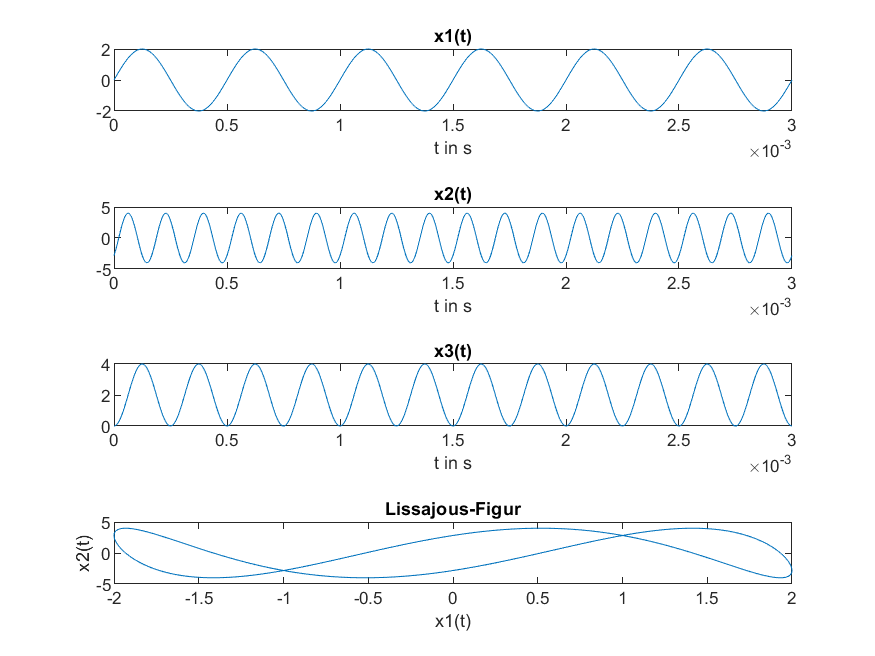
\includegraphics[width=\imagewidth]{../versuch1/sinus}
        \caption{Darstellung der Sinussignale}
        \legend{\(10^3\) Abtastpunkte}
        \label{fig:sinus}
    \end{figure}

    Wird der Zeitbereich der Lissajous-Figuren jedoch auf \SIrange{0}{3}{\second} gelegt und somit die Größenordnung um \(10^3\) erhöht, bleibt das Bild aufgrund des Aliasing-Effekts identisch. Wird der Zeitbereich leicht verschoben, entsteht ein nicht interpretierbares Bild. Beide Änderungen sind in Abbildung \ref{fig:lissajous} gezeigt. Der Code zum Erstellen der Grafiken befindet sich im Anhang \ref{lst:sinus}.

    \begin{figure}[hbt]
        \centering
        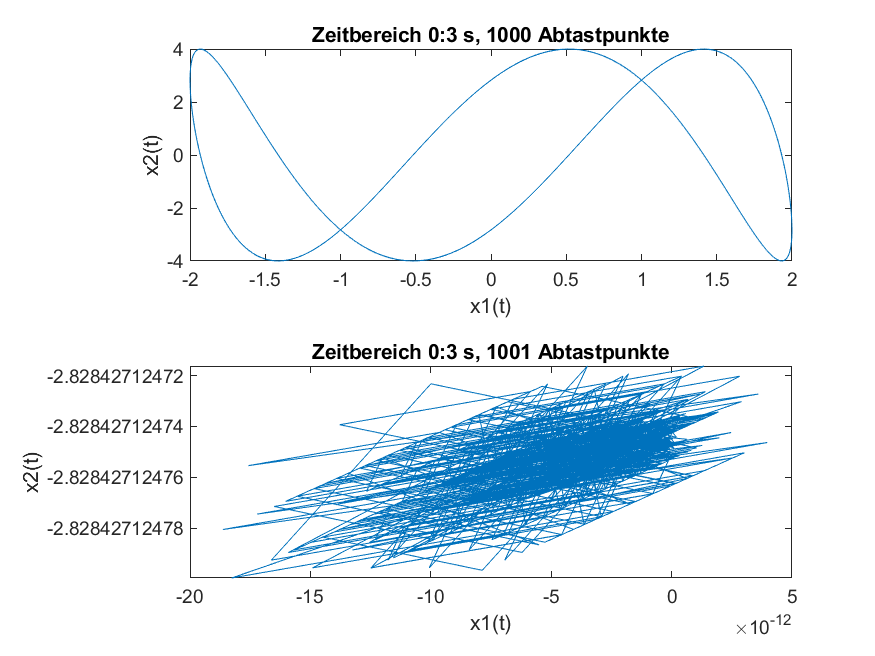
\includegraphics[width=\imagewidth]{../versuch1/lissjaou}
        \caption{Fehlerhafte Lissajous-Figuren}
        \label{fig:lissajous}
    \end{figure}

\section{Analyse eines Hochpasses}
    Zunächst werden die Bauteilwerte eines RC-Hochpasses bestimmt, bevor die Analyse mit MATLAB beginnt. Allgemein gilt für den Zusammenhang zwischen Eingangsspannung \(U_e\) und Ausgangsspannung \(U_e\) bei einem RC-Hochpass erster Ordnung:
    
    \begin{align}
        \label{eq:hochpass}
        \frac{U_a}{U_e} &= \frac{jwRC}{1+jwRC}
    \end{align}

    Und die Grenzfrequenz somit zu
    
    \begin{align}
        f_g &= \frac{1}{2 \pi R C}\\
        \intertext{Wird der Widerstand \(R\) auf \SI{1}{\kilo\ohm} und die Grenzfrequenz zu \SI{1e5}{\hertz} gewählt, berechnet sich die Kapazität zu:}
        C &= \frac{1}{2 \pi R f_g} = \SI{1.59e-9}{\farad}
    \end{align}

    Nun kann das vollständige Übertragungssystem in MATLAB verwendet werden. Das erzeugte Bodediagramm findet sich in Abbildung \ref{fig:bode} und die zugehörige Ortskurve in Abbildung \ref{fig:ortskurve}. Da die Ortskurve achsensymmetrisch zur x-Achse ist, kann das Diagramm ohne den Verlust von Informationen um genau diese Spiegelung verkürzt werden. Dies wird durch die Option \verb|ShowFullContour='off'| des \verb|nyquistplot|-Befehls erreicht. Der Code zum Erstellen der Diagramme findet sich in Anhang \ref{lst:tiefpass}.

    \begin{figure}
        \centering
        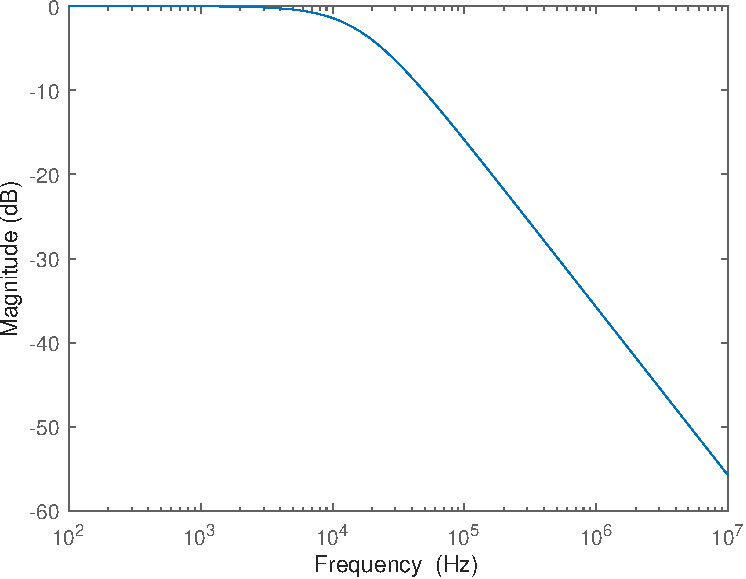
\includegraphics[width=\imagewidth]{../versuch1/bode}
        \caption{Bodediagramm des Hochpasses}
        \label{fig:bode}
    \end{figure}

    \begin{figure}
        \centering
        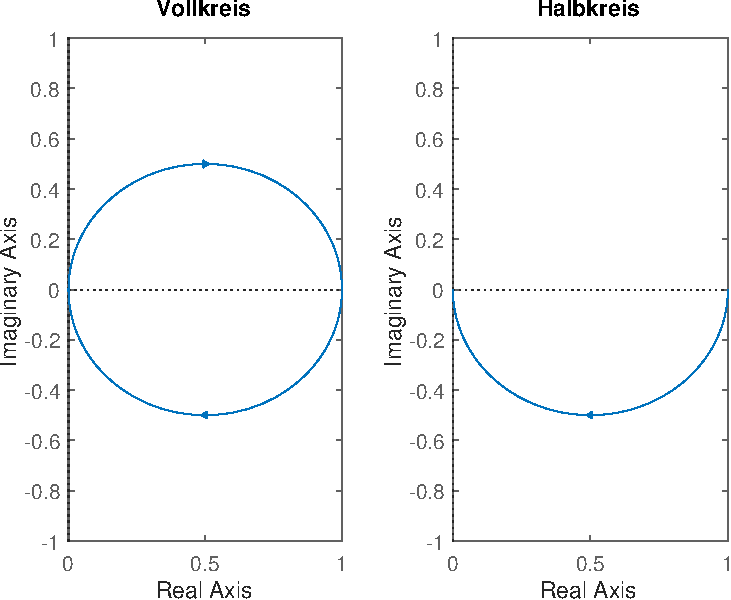
\includegraphics[width=\imagewidth]{../versuch1/ortskurve}
        \caption{Ortskurven des Hochpasses}
        \label{fig:ortskurve}
    \end{figure}

    \subsection{Nachweis der Kreisfunktion}

    Die Abbildung \ref{fig:ortskurve} zeigt einen Kreis mit Radius 0.5 und dem Mittelpunkt \complexnum{0.5 +0i}. Folgende Rechnung bringt den Nachweis, dass es sich tatsächlich um einen Kreis handeln muss..

    Für einen Kreis mit Mittelpunkt \(m\), sowie Radius \(r\), gilt in der komplexen Zahlenebene mit der Variablen \(z \in \mathbb{C}\):
    
    \begin{align}
        \left| z - m \right| = r
    \end{align}

    Einsetzen der Gleichung \eqref{eq:hochpass} für \(z\) und \(m= 0.5 +0i\) ergibt:

    \begin{align}
        \left|\frac{jwRC}{1+jwRC} - \complexnum{0.5 +0i} \right| = \left| \frac{1}{2} \cdot \frac{-1 + jwRC}{1 + jwRC} \right| = \left| \frac{1}{2} \cdot \frac{(wRC)^2 - 1}{(wRC)^2 + 1} + i \frac{wRC}{(wRC)^2 + 1} \right| \\
        = \sqrt{ \frac{1}{4} \left( \frac{(wRC)^2 - 1}{(wRC)^2 + 1} \right)^2 + \frac{1}{4} \left( \frac{2wRC}{(wRC)^2 + 1} \right)^2} = \frac{1}{2} \sqrt{ \frac{ \left(\left(wRC\right)^2 - 1\right)^2 + 4 (wRC)^2 }{\left(\left(wRC\right)^2 + 1\right)^2} } = \frac{1}{2}
    \end{align}

    \clearpage

\section{Temperaturregler mit SIMULINK}
    Zuletzt wird der Temperaturregler für einen Backofen betrachtet. Aus der Aufgabenstellung \cite{versuch1} wird das Blockschaltbild in SIMULINK erzeugt (siehe Abbildung \ref{fig:tempregler_block}). Der Puls-Generator am Eingang simuliert das Einschalten auf eine Solltemperatur von \SI{160}{\celsius} zu Beginn der Simulation und das Ausschalten nach \SI{30}{\minute}. Mit dem Parameter \(K_1\) wird diese Temperatur zu einem Spannungswert übersetzt. Der Zweipunktregler schaltet bei der Spannung \(u_{ein}\) ein und gibt eine Spannung von \SI{230}{\volt} aus. Bei einer Eingangsspannung von \(u_{aus}\) schaltet er ab. Das Heizgerät wird mit einem PT1-Glied simuliert. Dabei wird mit \(K_2\) das Ergebnis wiederum als Temperatur zurückgerechnet. Die Werte der einzelnen Simulationswerte sind in Tabelle \ref{tab:tempregler} gezeigt. 

    \begin{table}[hbt]
        \centering
        \caption{Parameter des Temperaturreglers}
        \label{tab:tempregler}
        \begin{tabular}{lr}\toprule
            Parameter   &   Wert\\\midrule
            \(K_1\)     & \SI{0.025}{\volt\per\celsius}\\\addlinespace
            \(K_2\)     & \SI{1,739}{\celsius\per\volt}\\\addlinespace
            \(u_{ein}\) & \SI{0.2}{\volt}\\
            \(u_{aus}\) & \SI{-0.2}{\volt}\\
            timeconst   & \SI{15}{\minute}\\\bottomrule
        \end{tabular}
    \end{table}
    
    Somit ist die Solltemperatur die Führungsgröße, die Eingangsspannung am Zweipunktegler entspricht der Stellgröße und die Ausgangstemperatur des Heizelements ist die Regelgröße. Der zeitliche Verlauf dieser Variablen über \SI{70}{\minute} ist in Abbildung \ref{fig:tempregler_plot} dargestellt. Durch Verändern der Schaltschwelle zu  \(\pm\SI{0.01}{\volt}\) erhält man Abbildung \ref{fig:tempregler_plot_new}.

    \begin{figure}
        \centering
        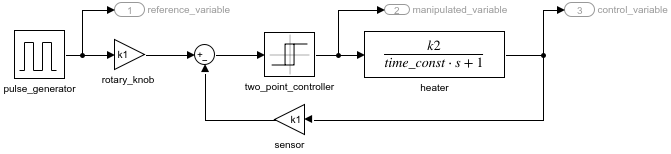
\includegraphics[width=\imagewidth]{../versuch1/tempregler_block.png}
        \caption{Blockschaltbild des Temperaturreglers}
        \label{fig:tempregler_block}
    \end{figure}    

    Aus den Abbildungen ist zu erkennen: Wird die Differenz zwischen Soll- und Ist-temperatur zu groß, wird die Schaltschwelle \(u_{ein}\) überschritten und der Zweipunktegler aktiviert die Heizung. Bei umgekehrten Vorzeichen wird die Heizung ausgeschalten. Durch Verkleinern der Schaltschwelle wird der Regler häufiger umschalten und die Ist-Temperatur weicht weniger von der Führungsgröße ab. Der Code zum Darstellen der Ergebnisse findet sich in \ref{lst:tempregler}.

    \begin{figure}
        \centering
        \begin{subfigure}{0.49\columnwidth}
            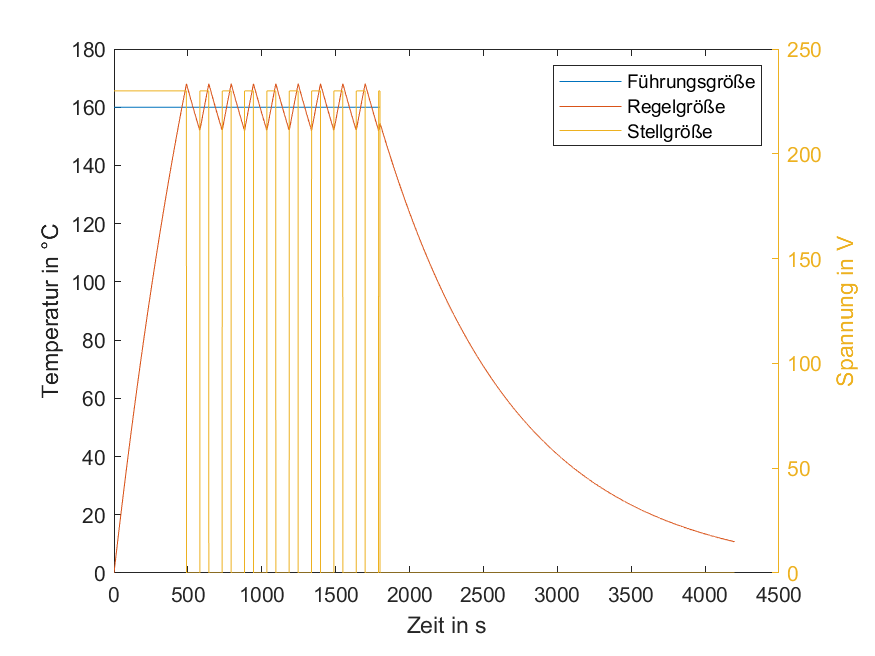
\includegraphics[width=1.0\columnwidth]{../versuch1/tempregler_plot.png}
            \caption{Schaltschwelle \(\pm\SI{0.2}{\volt}\)}
            \label{fig:tempregler_plot}   
        \end{subfigure}%
        \hfill%
        \begin{subfigure}{0.49\columnwidth}
            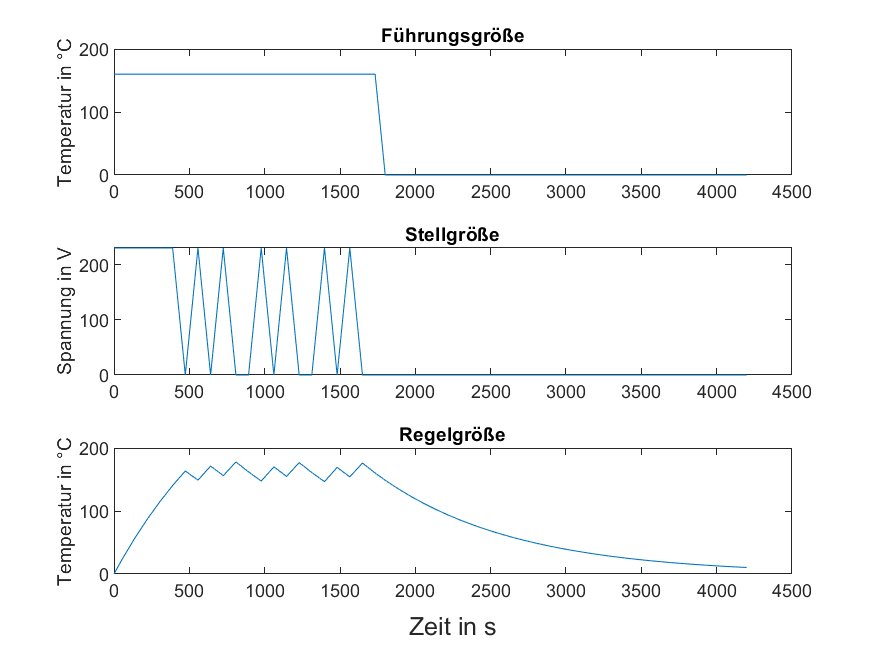
\includegraphics[width=1.0\columnwidth]{../versuch1/tempregler_plot_new.png}
            \caption{Schaltschwelle \(\pm\SI{0.01}{\volt}\)}
            \label{fig:tempregler_plot_new}
        \end{subfigure}
        \caption{Zeitliche Darstellung der Regelgrößen}
    \end{figure}

%-------------------------------------------------------------------------------------------------
%   Bibliography
%-------------------------------------------------------------------------------------------------

\printbibliography[heading=bibnumbered]

\section{Autorenbeiträge}
    Maileen Schwenk und Jan Hoegen erstellten die Vorbereitung und Messauswertung. Jan Hoegen schrieb den Bericht.

\section{Verfügbarkeit des Codes}
    Der Code zum Auswerten der Daten und Erstellen der Diagramme findet sich unter \url{https://github.com/JaxRaffnix/Regelungstechnik}. Ebenfalls ist hier der Code zum Erstellen dieser Ausarbeitung hinterlegt.

%-------------------------------------------------------------------------------------------------
%   Appendix
%-------------------------------------------------------------------------------------------------

\appendix

\section{MATLAB-Code der Sinussignale}
    \lstinputlisting[language=MATLAB, label={lst:sinus}]{../versuch1/sinus.m}

\section{MATLAB-Code zum Tiefpass}
    \lstinputlisting[language=MATLAB, label={lst:tiefpass}]{../versuch1/hochpass.m}

\section{MATLAB-Code zum Temperaturregler}
    \lstinputlisting[language=MATLAB, label={lst:tempregler}]{../versuch1/tempregler.m}

\end{document}